%\chapter{UML}
\section{Outil de modélisation}
\subsection{Intérêt d'une modélisation}
Un modèle est une représentation abstraite et simplifiée d'une entité du monde réel en vue de le décrire, de l'expliquer ou de le prévoir. Modéliser, c’est décrire de manière visuelle et graphique les besoins et les solutions fonctionnelles et techniques d'un projet.\\
Concrètement, un modèle permet de réduire la complexité d'un phénomène ou d'une entité en éliminant les détails qui n'influent pas son comportement de manière significative. Il reflète ce que le concepteur croit important pour la compréhension et la prédiction du phénomène modélisé. Les limites du phénomène modélisé dépendent des objectifs du modèle.\\
Modéliser un système avant sa réalisation permet de mieux comprendre le fonctionnement du système. C’est également un bon moyen de maîtriser sa complexité et d’assurer sa cohérence. Un modèle est un langage commun, précis, qui est connu par tous les membres de l’équipe et il est donc, à ce titre, un vecteur privilégié pour communiquer. Cette communication est essentielle pour aboutir à une compréhension commune  et précise d'un système par ses différentes parties prenantes.
\subsection{Présentation d'UML}
UML est l’acronyme de « Unified Modeling Langage » \nomenclature{UML}{Unified Modeling Language} qu'on peut traduire par « langage de modélisation unifié ». Il s'agit d'un langage de modélisation graphique et textuel, un outil de modélisation constitué d’un ensemble de schémas, appelés diagrammes UML, qui donnent chacun une vision différente du projet à traiter. En effet, un document texte décrivant de façon précise un système contiendrait plusieurs pages. En général, peu de personnes ont envie de lire ce genre de document. De plus, un long texte de plusieurs pages est source d’interprétations et d’incompréhension. UML nous aide à faire cette description de façon graphique et devient alors un excellent moyen pour « visualiser » le futur système.\\
UML utilise l'approche objet qui a déjà fait ses preuves. Il permet de faire une abstraction des technologies objet en permettant d’exprimer et d’élaborer des modèles objet, indépendamment de tout langage de programmation. L'aspect formel de sa notation, limite les ambiguïtés et les incompréhensions.\\
Son indépendance par rapport aux langages de programmation, aux domaines d'application et
aux processus, en fait un langage universel. En effet, le processus de collecte et d'analyse des exigences d'une application et de leur intégration dans la conception d'un programme, est complexe et il existe actuellement nombre de  méthodologies qui définissent des procédures formelles spécifiant la démarche à suivre. Une des caractéristiques d'UML est qu'il est indépendant de toute méthodologie. Quelle que soit la méthodologie de développement utilisée dans un projet, on peut utiliser UML pour la modélisation du système. Il a été pensé pour servir de support à une analyse des concepts objet. C’est un langage formel, défini par un méta-modèle.\\
UML est aussi un support de communication performant, qui facilite la compréhension de systèmes  aussi complexes qu'ils soient.\\
UML est le résultat de la fusion de trois méthodes orientées objet Booch, OMT (Object Modeling Technique) et OOSE (Object Oriented Software Engineering) \nomenclature{OMT}{Object Modeling Technique} \nomenclature{OOSE}{Object Oriented Software Engineering} conçues respectivement par Grady Booch, James Rumbaugh et Ivar Jacobson. UML a démarré avec la version 0.8 intégrant les méthodes BOOCH 93 et O.M.T. Par la suite ce fut l'avènement de la version 0.9 ayant intégré la méthode OOSE. La version 1.0, proposé à l'O.M.G en 1996, fut finalement standardisée en 1997 sous la version 1.1 . Depuis, il y a eu plusieurs révisions du standard. Les dernières améliorations étant conséquentes, UML est passé à une nouvelle version : UML 2.0 (ou UML 2), abrégé souvent en U2. En 2005, l'Organisation internationale de normalisation (ISO) a également publié UML en tant que norme ISO approuvée.Actuellement, UML en est à sa version 2.5.
\subsection{Diagrammes UML}
UML propose 14 diagrammes qui sont dépendants hiérarchiquement et se complètent, de façon à permettre la modélisation d'un projet tout au long de son cycle de vie. Un diagramme UML est une représentation graphique, qui s'intéresse à un aspect précis du modèle. C'est une perspective du modèle. Ces diagrammes sont répartis en 3 grands groupes :
\begin{itemize}
	\itemcheck Diagrammes structurels ou statiques qui s'intéressent la structure interne du système :
	\begin{itemize}
		\itemtirait Diagramme de classes : il représente les classes intervenant dans le système et les associations, agrégations, généralisation, interfaces, etc... ;
		\itemtirait Diagramme d'objets : il sert à représenter les instances de classes (objets) utilisées dans le système ;
		\itemtirait Diagramme de composants : il permet de montrer les composants du système d'un point de vue physique ;
		\itemtirait Diagramme de déploiement : il sert à représenter les éléments matériels et la manière dont les composants du système sont répartis sur ces éléments matériels et interagissent entre eux ;
		\itemtirait Diagramme de paquetages : il sert à représenter les dépendances entre paquetages, c’est-à-dire les dépendances entre ensembles de définitions ;
		\itemtirait Diagramme de structure composite : il montre l’organisation interne d’un élément statique complexe ;
		\itemtirait Diagramme de profils : il permet de spécialiser, de personnaliser pour un domaine particulier un méta-modèle de référence d'UML.
	\end{itemize}
	\itemcheck Diagrammes comportementaux qui s'intéressent aux interactions du système, avec lui même et avec d'autres entités : 
	\begin{itemize}
		\itemtirait Diagramme des cas d'utilisation : il représente la structure des grandes fonctionnalités nécessaires aux utilisateurs du système ;
		\itemtirait Diagramme d'états-transitions : il représente la façon dont évoluent les objets appartenant à une même classe ;
		\itemtirait Diagramme d'activités : le diagramme d'activités n'est autre que la représentation du processus tel qu'il a été élaboré lors du travail qui a préparé la modélisation : il montre l'enchaînement des activités qui concourent au processus.
	\end{itemize}
	\itemcheck Diagrammes d’interaction ou dynamiques :
	\begin{itemize}
		\itemtirait Diagramme de séquence : il permet de décrire séquentiellement les différents scénarios d’utilisation du système ;
		\itemtirait Diagramme de communication : c’est la représentation simplifiée d'un diagramme de séquence se concentrant sur les échanges de messages entre les objets ;
		\itemtirait Diagramme global d'interaction : permet de donner une vue d’ensemble des interactions du système. Il est réalisé avec le même graphisme que le diagramme d’activités ;
		\itemtirait Diagramme de temps : il permet de décrire les variations d'un objet au cours du temps.
	\end{itemize}
\end{itemize}
\begin{figure}[h!]
	\centering
	\begin{minipage}{18cm}
		\centering
		{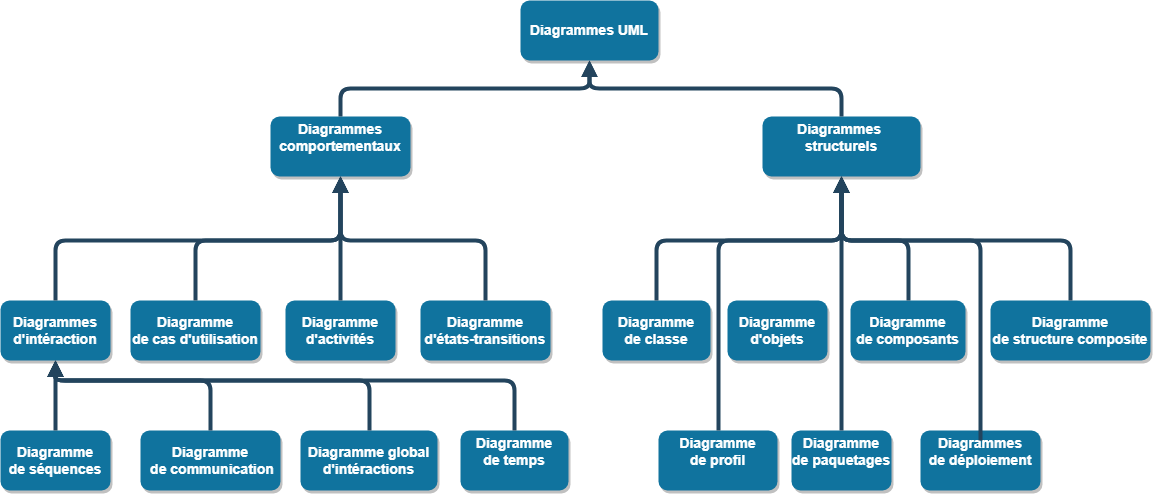
\includegraphics[height=0.27\textheight]{fig/Uml-Diagrams-overview.png}}
	\end{minipage}
	\caption{Schéma d'ensemble des diagrammes UML}
	\label{fig:7.1}
\end{figure}
La figure \ref{fig:7.1} une vue globale et hiérarchique des quatorze diagrammes UML.\\
Ces diagrammes, d'une utilité variable selon les cas, ne sont pas nécessairement tous produits à l'occasion d'une modélisation. Nous utiliserons au besoin certains de ces diagrammes pour illustrer les aspects de notre solution.

\clearpage 

